\newcommand{\CLASSINPUTbaselinestretch}{0.92}
\documentclass[conference]{IEEEtran}

%%%%%%%%%%%%%%%%%%%%%%%%%%%%%%%%%%%%%%%%%%
%%% 次回以降の原稿執筆時の注意点まとめ %%%
%%%%%%%%%%%%%%%%%%%%%%%%%%%%%%%%%%%%%%%%%%
%%
% Distribution information が企業間の競争優位を築く理由、二次流通市場の個人間の流通情報を含む理由は、shortpaperなので省略しているけど、Reviewerからツッコミが入るかもしれない。
%%
% fullpaperや国内会議原稿を書くときには、なぜmanufacturerの公開鍵で暗号化するのか(もっといえば、なぜmanufacturerのみが追跡できればよいのか)をしっかり論じる必要がある。securing traceability by the manufacturer と急にでてくるので、読んでる方は結構ドキッとする。
%%
% Zero-Knowledge Proofを使う時の public と private の input として何を使っているのか明記したほうがいい。
%

% packages
\usepackage{cite}
\usepackage{amsmath}
\interdisplaylinepenalty=2500
% \usepackage{fixltx2e}
\usepackage{stfloats}
\fnbelowfloat
\usepackage{url}


\ifCLASSINFOpdf

\else
    % \usepackage[dvips]{graphicx}
    % \usepackage[dvipdfmx]{graphicx}
    \usepackage{graphicx}
    % \graphicspath{{./figure/}}
\fi

\hyphenation{op-tical net-works semi-conduc-tor}


\begin{document}
%
% paper title
% can use linebreaks \\ within to get better formatting as desired
\title{Short Paper: Design and Evaluation of Privacy-preserved 
Supply Chain System\\ based on Public Blockchain}


% author names and affiliations
% use a multiple column layout for up to three different
% affiliations

\author{
    \IEEEauthorblockN{Takio Uesugi\IEEEauthorrefmark{1},
        Yoshinobu Shijo\IEEEauthorrefmark{1}, 
        Masayuki Murata\IEEEauthorrefmark{1}
    }
    \IEEEauthorblockA{
        \IEEEauthorrefmark{1}Graduate School of Information Science and Technology, Osaka University \\
        1--5 Yamadaoka, Suita, Osaka, 565--0871 Japan\\
        Email: \{t-uesugi, y-shijo, murata\}@ist.osaka-u.ac.jp
    \vspace{-1pt}} % title area と main text の感覚詰める
}

% use for special paper notices
%\IEEEspecialpapernotice{(Invited Paper)}

% make the title area
\maketitle


\begin{abstract} %\boldmath
% サプライチェーンにおける製品の追跡性を確保することは喫緊の課題である。
% 近年、Public Blockchain(PBC)を利用したサプライチェーンシステムが提案されている。
% これらシステムでは、PBCを事業者間の共通データベースとして使うことによって、例えば所有者の移転記録などの流通情報の完全性と真正性を担保する。
% そのため、高い追跡性を確保することができる。
% しかし一方で、PBCに記録されている情報は誰でも閲覧可能であるため、プライバシー情報である流通情報が公開されてしまう。
% そこで、本研究では、PBCを利用したサプライチェーンシステムにおいて、追跡性を担保しつつも、プライバシーを保護可能な手法を提案する。
% 提案手法では、流通情報を暗号化によって隠蔽することでプライバシーを保護する。
% また、ゼロ知識証明に基づいて正規の流通者であることを証明することで、ブロックチェーンアドレスを隠蔽しつつも、正規の流通者間での流通を保証する。
% 提案手法を Ethereum のスマートコントラクトで実装し、トランザクション手数料に基づくコスト評価を実施する。
% その結果、流通者あたりの手数料は高々 2.6 USD 負担であることを示す。
Securing the traceability of products in the supply chain is an urgent issue.
Recently, supply chain systems that use public blockchain (PBC) have been proposed.
In these systems, PBC is used as a common database shared between %\todo{distributors}
supply chain parties to secure the integrity and reliability of distribution information such as ownership transfer records.
Thus, %they
these systems secure a high level of traceability in the supply chain.
However, the distribution information, which can be private information, is made public since the information recorded in PBC can be read by anyone.
In this paper, we propose a method for preserving privacy while securing traceability in a supply chain system using PBC.
The proposed method preserves privacy by concealing the distribution information via encryption.
In addition, the proposed method ensures distribution among legitimate %distributors
supply chain parties while concealing their blockchain address by using a zero-knowledge proof to prove their authenticity. %legitimacy.
We implement the proposed method on Ethereum smart contracts and evaluate cost performance based on transaction fees.
The results show that the fee per %distributor 
party is at most 2.6 USD.
\end{abstract}

% For peer review papers, you can put extra information on the cover
% page as needed:
% \ifCLASSOPTIONpeerreview
% \begin{center} \bfseries EDICS Category: 3-BBND \end{center}
% \fi
%
% For peerreview papers, this IEEEtran command inserts a page break and
% creates the second title. It will be ignored for other modes.
\IEEEpeerreviewmaketitle

\section{Introduction}

\begin{figure*}[b]
    \centering
    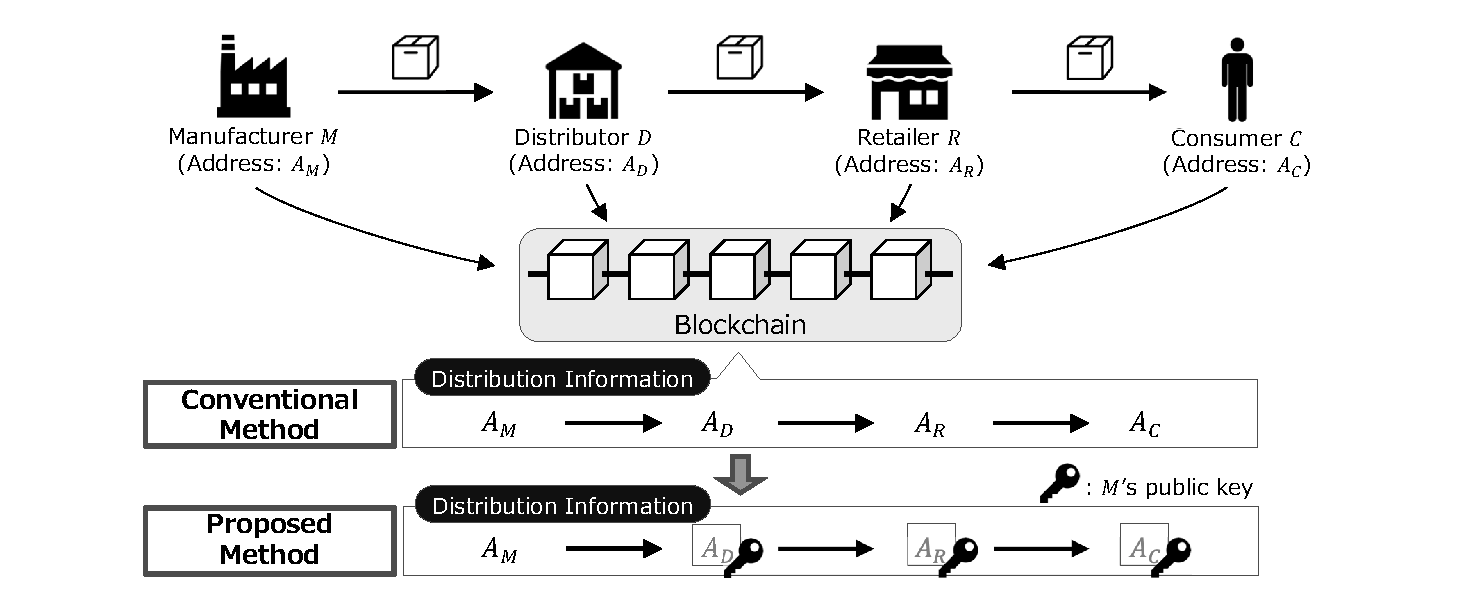
\includegraphics[width=0.74\textwidth]{outline.eps}
    \caption{Overview of conventional and proposed methods.
    \label{fig:outline}}
\end{figure*}

%% 四條メモ: アドレスと実世界でのエンティティが繋がっていることを指摘する

% %% 本論文の背景
% %% サプライチェーンシステムの追跡性が困難になってきている→問題が顕在化している
% 近年、サプライチェーンのグローバル化が急速に進んでおり、特に製品の追跡性に関して深刻な問題が発生してきている。
% 例えば、製品製造者の真正性の確認が困難になりつつあるため、偽造品の流通額は2013年に4610億米ドルだったのに対し、2016年には5090億米ドルまで増加している~\cite{OECD/EUIPO2019}。
% また、食中毒を引き起こしている食品の所在の特定ができず、食中毒被害が広がってしまった事例もある~\cite{chipotle}。
Rapid globalization of supply chains has led to serious problems, particularly with respect to traceability.
The Organisation for Economic Co-operation and Development (OECD) reported that counterfeit products in international trade totaled 509 billion USD in 2016, up from 461 billion USD in 2013~\cite{OECD/EUIPO2019}.
% Furthermore, a lack of traceability in complex supply chain led to the 2015 E.coli outbreak at Chipotle Mexican Grill~\cite{chipotle}.
Furthermore, due to the complexity of the supply chain, ingredients contaminated with \textit{Escherichia coli} could not be tracked, resulting in the 2015 \textit{E. coli} outbreak at Chipotle Mexican Grill~\cite{chipotle}.

% %% 解決策(既存手法)
% %% ブロックチェーンを利用したサプライチェーン管理システム
% %%% 「流通情報」の定義を明確に
% こうした課題を解決するために、ブロックチェーンを利用したサプライチェーンシステムが提案されている~\cite{Toyoda2017, TRU, HZL19}。
% これらシステムでは、製品の流通情報をパブリックブロックチェーンに保存する。
% ここで流通情報とは、所有者の移転記録である。
% また、スマートコントラクトを活用することで、流通情報の登録に適切な条件を設けることによって、不正な流通情報の登録を防ぐ。
% 一度ブロックチェーンに保存された流通情報は、ブロックチェーンの改ざん耐性により、変更することはできない。
% そのため、高い追跡性を確保することができる。 
% なお、所有者はブロックチェーンアドレスを用いて管理される。
% 一般に、ブロックチェーンアドレスと実世界のエンティティは結びついていないため、公開鍵証明書と同様の仕組みを用いることで、企業あるいは個人の情報とブロックチェーンアドレスを一意に対応付ける。
To remedy these problems, supply chain systems based on blockchain have been proposed~\cite{Toyoda2017, TRU, HZL19}.
% These systems store distribution information of the products, which is the record of the owner transfers, in a public blockchain.
These systems store distribution information of products in a public blockchain (PBC).
Note that the distribution information in these systems are the records of ownership transfers.
Smart contracts prevent the registration of fraudulent distribution information by setting appropriate conditions.
Once information has been stored in the blockchain, no one can alter the information due to its immutability.
Therefore, these systems secure a high level of traceability in the supply chain.
Note that owners are managed by using their blockchain addresses.
In general, blockchain addresses are not tied to real-world entities.
Thus, a mechanism similar to public key certificates is used to link blockchain addresses to information about a company or individual.

% %% 既存手法の問題
% %% プライバシーの問題
% %%%  「プライバシー」の定義を明確に
% しかしながら、これらの手法にはプライバシーの問題がある。
% パブリックブロックチェーンでは、誰でも自由に保存されている情報を閲覧できる。
% そのため、競争優位を築いている企業間の流通情報や、二次流通市場における個人間の流通情報など、秘匿されるべき情報までもが公になってしまう。
% よって、流通情報はプライバシー情報であり、保護する必要がある。

% しかしながら、これらの手法にはプライバシーの問題がある。
% 流通情報は、企業間の競争優位を築いていたり、あるいは二次流通市場における個人間の関係を含む。
% そのため、流通情報はプライバシー情報であり、保護する必要がある。
% 一方で、パブリックブロックチェーンでは、誰でも自由に保存されている流通情報を閲覧できる。
% そのため流通情報のプライバシーが保護されない。
However, there are privacy issues with these systems.
Distribution information is part of the competitive advantage of companies, and may include relationships between individuals in secondary markets.
Therefore, distribution information is private information that needs to be protected.
However, information recorded in a PBC can be freely viewed by anyone.
As a result, the privacy of distribution information is not protected.

% However, there are privacy issues with these systems.
% % In a public blockchain, anyone can view its stored information freely.
% As information recorded in public blockchain can be freely viewed by anyone,
% distribution information that should be kept confidential becomes public.
% For example, these are business relationship between companies, which has competitive advantages in business, and personal relationship between individuals in the secondary market.
% Therefore, the distribution information is privacy information and needs to be preserved.

% %% 提案手法
% %% 何を実現しているのか?
% %% 手法の中で特筆すべき工夫、アピールポイントがあれば端的に書く。
% そこで本研究では、パブリックブロックチェーンを利用したサプライチェーンシステムにおいて、製品製造者による追跡性を担保しつつも、プライバシーを保護可能な手法を提案する。
% 既存手法がプライバシーを毀損している要因は、ブロックチェーンアドレスを直接ブロックチェーンに保存していることにある。
% そこで我々の手法では、図~\ref{fig:outline}のように、製造者の公開鍵を利用してブロックチェーンアドレスを暗号化し、それをブロックチェーンに保存することで、プライバシーを保護する。
% 製造者は、自身の秘密鍵を用いて復号し、アドレスを取得することで、流通経路を追跡できる。
% なお、不正な流通を排除するために、製品の発送・受領処理を実施する際には、自身が正規の流通者であることをシステムに示す必要がある。
% そこで提案手法では、ゼロ知識証明を利用することで、ブロックチェーンアドレスを隠蔽しつつも、自身の真正性の証明を可能にする。
In this paper, we propose a method for preserving privacy while securing traceability by the manufacturer of a product in supply chain systems that use PBC.
The main reason why conventional methods cannot preserve privacy is that they store the blockchain addresses directly in the blockchain.
Therefore, the proposed method preserves privacy by encrypting blockchain addresses by using the manufacturer's public key and storing the encrypted addresses in the blockchain, as shown in \figurename~\ref{fig:outline}.
The manufacturer can then track the product by decrypting the addresses using its own private key.
% In order to eliminate unauthorized distribution, it is necessary to prove to the system that they is an authorized distributor when shipment and receipt of the product.
To eliminate %unauthorized distribution, 
distribution by %non-legitimate
illegitimate %distributors,
parties, the %distributors, meaning the parties in the supply chain
supply chain parties such as \textit{M, D, R} and \textit{C} in \figurename~\ref{fig:outline} %,
must indicate to the system that they are legitimate %distributors 
parties when they ship and receive the product.
% The distributor means the party in the supply chain such as \textit{M, D, R} and \textit{C} in \figurename~\ref{fig:outline}.
Accordingly, the proposed method uses a zero-knowledge proof to allow %distributors
supply chain parties to prove their authenticity %itself
while hiding %its
their blockchain addresses.

% %% 評価結果
% %% 何がわかったのか?
% 提案手法の動作検証を行うために、Ethereum~\cite{Ethereum}を用いて、提案手法を実装した。
% 動作検証では、製造者を起点に6回の製品流通、すなわち所有者の移転を行なった。
% その結果、プライバシーを担保しつつも製造者による追跡性を担保できることがわかった。
% また、流通に要するトランザクション手数料を評価したところ、流通者あたりの手数料は高々 2.6 USDであることがわかった。
To evaluate %the result of its operation of 
%the operation of
the proposed method, % In order to verify the operation of the proposed method, 
we implement it on the Ethereum platform.
% The operation verification involves six times of distributions, or transfers of ownership, starting with the manufacturer.
We assume %six distributions
distributions of a product, or transfers of ownership, starting with the manufacturer %for
in the evaluation.
% in order to verify the operation.
% As a result, we validate that it is possible to secure the traceability by the manufacturer while preserving privacy.
The results show that the proposed method can preserve privacy while securing traceability by the manufacturer.
We also evaluate the transaction fees for distribution and find that the fee per %distributor
party is at most 2.6 USD.


% %% この後の論文構成
% %% 各セクションで何に言及しているのか?
% 以降の構成は次の通りである。
% 2章では関連研究を紹介し、3章では提案手法を説明する。
% 4章では、プライバシー担保と追跡性確保に関して、提案手法の有効性を検証する。
% 5章では、提案手法の実験環境の説明と動作検証の結果を説明する。また、トランザクション手数料の評価結果を示し、提案手法は高単価製品への適用が見込まれることを議論する。
% 最後に6章において、結論と今後の課題を述べる。
The rest of this paper is structured as follows.
Section \ref{sec:related_work} discusses related work.
Section \ref{sec:proposed_method} introduces the proposed method, which is verified in Section \ref{sec:verification} in terms of privacy and traceability.
% Section \ref{sec:evaluation} describes the experimental environment of the proposed method and the result of its operation verification.
Section \ref{sec:evaluation} describes the environment for evaluating the proposed method and presents the evaluation results. %the operational verification of the proposed method.
We also present the results of evaluating transaction fees.
% Finally,
Lastly, our conclusions and future work are presented in Section \ref{sec:conclusions}.


\section{Related Work}
\label{sec:related_work}
% サプライチェーンにおける製品の追跡性の向上を目的に、ブロックチェーンを活用したシステムがいくつか提案されてきている。
% 文献~\cite{Toyoda2017}では、ポストサプライチェーンにおける偽造品流通の防止を目的として、製品の所有者の変遷をブロックチェーンを用いて管理するための手法を提案している。
% また、文献~\cite{TRU}では、流通に関与する製品やその材料を Traceable Resource Unit (TRU) とみなし、これの消費・生産を繰り返すことで、材料から製品に至るまでの流通経路の追跡を可能にする手法を提案している。
% 文献~\cite{HZL19}は、オフチェーン技術を活用することで、高頻度で流通が行われるフードサプライチェーンに適用可能な手法を提案している。
% しかしながら、いずれの手法においても流通情報のプライバシー保護は検討されていない。
% 我々が知る限り、我々の提案手法は、パブリックブロックチェーンを用いたサプライチェーンシステムにおいて、追跡性の担保とプライバシーの保護を両立可能な世界初の方法である。
Several blockchain-based systems have been proposed for improving the traceability of products in supply chains.
POMS~\cite{Toyoda2017} is a system for managing product ownership using the blockchain to prevent distribution of counterfeits in the post-supply chain.
Kim et al.~\cite{TRU} proposed a method for tracking products from the materials stage by repeated consumption and production of traceable resource units (TRUs).
Huang et al.~\cite{HZL19} proposes a method that can be applied to the food supply chain, which features high-frequency distribution, through the use of off-chain technology.
However, the protecting the privacy of distribution information has not been considered in any methods.
% To our knowledge, the proposed method is the first in the world to ensure both traceability and privacy in supply chain system using PBC.




\section{Proposed Method}
\label{sec:proposed_method}

% 提案手法は、文献~\cite{Toyoda2017}の手法をベースとし、流通情報のプライバシーを担保する方法を追加する。
% 提案手法では、製造者の公開鍵を利用してブロックチェーンアドレスを暗号化する。これをブロックチェーンに保存することで、ブロックチェーンアドレスを隠蔽し、プライバシーを保護する。
% 製造者は、自身の秘密鍵で復号することでブロックチェーンアドレスを取得し、流通を追跡できる。
% また、ゼロ知識証明に基づき、正規の流通者のみが持つ Secret Token を知っていることを示す証明を行うことで、ブロックチェーンアドレスを隠蔽しつつも、正規の流通者間での流通を保証する。
We propose a method for preserving the privacy of distribution information %based on POMS
by extending POMS~\cite{Toyoda2017}.
The proposed method uses the public key of the product manufacturer to encrypt blockchain addresses.
Storing these encrypted addresses in the blockchain conceals the blockchain addresses and preserves privacy.
A manufacturer can track its products by using its own private key to decrypt and get the list of the blockchain addresses.
In addition, each of the %distributors
supply chain parties proves, based on a zero-knowledge proof, that it knows a secret token possessed by only legitimate %distributors
supply chain parties.
Thus, the proposed method ensures distribution among legitimate %distributors
supply chain parties while concealing their blockchain addresses.

% 提案手法は、製造者情報を管理するスマートコントラクト\textit{ManufacturersManagerContract(MMC)}と、製品流通を管理するスマートコントラクト\textit{ProductsManagerContract(PMC)}、ゼロ知識証明の証明情報の検証を行なうスマートコントラクト\textit{VerifierContract(VC)}から構成される。
% 以降では、これら3つのスマートコントラクトを利用した、流通の事前準備、製品の登録、製品の流通処理、製品の追跡方法について説明する。
The proposed method consists of \textit{ManufacturerManagerContract (MMC)} for managing manufacturer information, \textit{ProductsManagerContract (PMC)} for managing product distributions, and \textit{VerifierContract (VC)} for verifying a proof based on the zero-knowledge proof.
In the following, we describe how to use these three contracts to prepare for distribution, register a product, manage distribution, and track the product.

\subsection{Preparation for distribution}
% 流通の事前準備として、MMCに製造者情報を登録する。
% 必須の情報は、製造者のブロックチェーンアドレスと公開鍵の組である。
% 必要に応じて、製造者の名前や住所なども登録することができる。
% この登録処理は、指定された管理者のみが実行可能である。
% 例えば、サプライチェーンの国際規格の設計・策定を行っている非営利組織GS1~\cite{GS1}が行うことが想定される。
To prepare for distribution, the manufacturer information is registered in \textit{MMC}.
The required information is a pair consisting of the manufacturer's blockchain address and public key.
Other information such as the name and phone number of the manufacturer % The name and \comu{street} address of the manufacturer
can also be registered if necessary.
In addition, \textit{MMC} associates the manufacturer's blockchain address with its products.

These %This
registration processes %process
can be executed only by a designated administrator.
For example, this could be performed by GS1~\cite{GS1}, an NPO that develops and maintains global standards for supply chains.

% \comu{\textit{MMC} associates the manufacturer's blockchain address with its product.
% If the manufacturer registers a product with the \textit{PMC}, \textit{PMC} confirms the product that the manufacturer is trying to register is associated in \textit{MMC}.}

\subsection{Products registration}
% MMCに登録されている製造者のみが、製品の最初の所有者として、PMCに製品を登録することができる。
% なお、製品と製造者はMMCで対応付けられており、製造者がPMCに登録可能な製品は限定されていることとする。
% 製品の流通は、MMCに登録された製造者であること、およびその製造者の製品であることを確認した後、PMCに製品情報を登録することで、開始される。
% 以降、PMCを用いて所有者を管理する。
Only a manufacturer registered with \textit{MMC} can register its products with \textit{PMC} as the first owner of the product.
% The products and the manufacturer are associated in \textit{MMC} in advance,
% \coms{and the products that the manufacturer can register with \textit{PMC} are restricted.}
% the products that the manufacturer can register are limited.
% the manufacturer can register only its own products with \textit{PMC}.
% Distribution of a product is initiated by registering the product information with \textit{PMC} after confirming that %it
% \comu{the party registering the product} is a manufacturer registered with \textit{MMC} and that it is a product of the manufacturer.
Distribution of a product is initiated by a manufacturer's registration of the product information with \textit{PMC} after confirmation that the manufacturer is registered with \textit{MMC} and is associated with the product.
Below, \textit{PMC} is used to manage ownership.

% 製造者のみ、PMCには暗号文ではなくアドレスを記録する。
% これは、製造者は自身が製品を製造したことを証明したい立場であり、隠蔽すべき対象でないためである。
% また、流通者は、PMCの初期所有者を見ることで、製品の製造者を自由に確認できる。
\textit{PMC} records the raw blockchain address, not the encrypted address, for the manufacturer only.
% Only the manufacturer records its blockchain address, not an encrypted address, in \textit{PMC}.
This is because the manufacturer would like to prove that it has manufactured the product.
%Distributors
Anyone can freely identify the manufacturer of the product by viewing the first owner recorded in \textit{PMC}.


\subsection{Distribution management}
% 図~\ref{fig:flow-ProposedMethod}は、流通管理全体の流れを図示している。
% 流通管理は次の8個のステップからなる。Step1から4が発送処理、Step5から8が受領処理である。
\figurename~\ref{fig:flow-ProposedMethod} illustrates the flow of distribution management.
Distribution management consists of the following eight steps: Steps~1 to~4 are the shipping process and Steps~5 to~8 are the receiving process.
\begin{enumerate}
    % \item 所有者は受領者に対して、Secret Token をセキュアな方法を用いて共有する。
    \item The owner shares a secret token with the recipient by a secure method.
    % \item 所有者は、Secret Tokenと製造者の公開鍵を用いて受領者のアドレス$A_R$を暗号化し、$Enc(A_R)$を得る。
    \item The owner encrypts the recipient's address $A_R$ using the secret token and the manufacturer's public key to obtain $\textit{Enc}(A_R)$.
    % \item 所有者は、 VC を登録する。
    \item The owner deploys \textit{VC} on the blockchain.
    % \item 所有者は、受領者のアドレスの暗号文$Enc(A_R)$とステップ3のVCのコントラクトアドレスを PMC に記録する。
    \item The owner records the recipient's encrypted address $\textit{Enc}(A_R)$ and the contract address of \textit{VC} obtained from Step~3 in \textit{PMC}.
    % \item 受領者は、ステップ1で共有されたSecret Tokenを知っていることを示す証明情報を、ゼロ知識証明に基づき生成する。
    \item The recipient generates a proof that it knows the secret token shared in Step~1 based on a zero-knowledge proof.
    % \item 受領者は、証明情報をPMCに送信する。
    \item The recipient sends the proof to \textit{PMC}.
    % \item PMC が VC を呼び出し、送信された証明情報が正しい証明であることを検証する。
    \item \textit{PMC} calls \textit{VC} and verifies that the proof sent is valid.
    % \item 所有者を$Enc(A_R)$に変更する。
    \item The owner is changed to $\textit{Enc}(A_R)$.
\end{enumerate}
% PMCは、これらステップのうち、Step 4, 6, 7, 8 の実行に必要な機能を提供する。
% 以降、重要なステップを取り上げ、説明を行う。
\textit{PMC} provides the necessary functions to perform Steps 4, 6, 7, and 8.
The important steps are explained below.

% まず、ステップ2のアドレスの暗号化について説明する。
% このアドレスの暗号化には次の式~(\ref{eq:ecelgamal})で表されるElliptic Curve Elgamal暗号を使用する。
First, we explain the encryption of the address in Step~2.
We use the elliptic curve elgamal encryption, as can be seen in (\ref{eq:ecelgamal}), to encrypt the address.
\begin{IEEEeqnarray}{rCl}
\textit{Enc}(A_R) = (kG, A_R + kQ) \label{eq:ecelgamal}
\end{IEEEeqnarray}
% 提案手法においては、$k$はSecret Token、$G$は楕円曲線の生成元、$A_R$は受領者のアドレス、$Q$は製造者の公開鍵である。
% 式~(\ref{eq:ecelgamal})を用いた暗号化を行なうためには、$A_R$は楕円曲線上の点である必要がある。
% そのため、実際は、$A_R$を楕円曲線上の点に変換した値を利用する。
In the proposed method, $k$ is the secret token, $G$ is the generator of the elliptic curve, $A_R$ is the recipient's address, and $Q$ is the manufacturer's public key.
Note that $A_R$ must be a point on the elliptic curve for encryption. % using (\ref{eq:ecelgamal}). 
Therefore, we use a value converted from $A_R$ to a point on the elliptic curve. %in practice.

% 次に、ステップ5のゼロ知識証明について説明する。
% 受領者アドレスの暗号文$Enc(A_R)$を計算するためには、式~(\ref{eq:ecelgamal})の$k,G,A_R,Q$を全て知っている必要がある。
% このうち、$G, A_R, Q$は公開情報であるから、$k$が所有者と受領者のみが知っている値である。
% つまり、$Enc(A_R)$を正しく計算できるのは、$k$を知っている正規の所有者と受領者のみである。
% よって、$Enc(A_R)$を計算できることを証明することで、自身が正規の受領者であることを示すことができる。
% 提案手法では、この証明にゼロ知識証明を利用する。
% これにより、$k$や$A_R$を明かすこと無く、$Enc(A_R)$を計算できることを証明できる。
% ゼロ知識証明には様々な実装があるが、本研究では、非対話式かつ証明サイズが小さいことから、ブロックチェーンとの相性が良いことが知られているzk-SNARKsを利用する~\cite{zk-SNARKsInBC}。
% この証明の検証は、ステップ~7で行われる。
% 証明の検証は、PMC が暗号文$Enc(A_R)$と公開鍵$Q$、ステップ5の証明情報を引数として、VCを呼び出して実行する。
% これにより、指定された暗号文を計算できることの証明のみが受理される。
Second, we describe the zero-knowledge proof in Step~5.
To calculate the recipient's encrypted address $\textit{Enc}(A_R)$, the owner and the recipient must know all of $k, G, A_R$ and $Q$ in (\ref{eq:ecelgamal}).
Although $G, A_R$ and $Q$ are public information, $k$ is known only to the owner and the recipient.
That is, only the legitimate owner and recipient who know $k$ can correctly calculate $\textit{Enc}(A_R)$.
Therefore, the recipient can prove that it is legitimate by proving that it can calculate $\textit{Enc}(A_R)$.
We use a zero-knowledge proof for this purpose.
Zero-knowledge proof allows the recipient to prove that it can calculate $\textit{Enc}(A_R)$ without revealing $k$ and $A_R$.
Although there are various implementations of zero-knowledge proofs, we utilize zk-SNARKs which is known to be compatible with blockchain due to its non-interactivity and small proof size~\cite{zk-SNARKsInBC}. 
This proof is verified in Step~7.
\textit{PMC} calls \textit{VC} with the recipient's encrypted address $\textit{Enc}(A_R)$, the manufacturer's public key $Q$, and the proof generated in Step~5 as arguments to verify this proof.
% As a result, only the proof of the %particular
% \comu{designated} encrypted address is accepted.

% 実際には、ステップ4においても、所有者であることを証明した後に、ブロックチェーンに受領者を記録する。
% これは、所有者以外による発送を防止するためである。
% 所有者であることの証明は、受領者であることを証明するときと同様に、所有者が暗号文$Enc(A_A)$を計算できることをゼロ知識証明する。
In practice, even in Step~4, the owner proves that it is legitimate before recording the recipient's encrypted address in \textit{PMC}.
This is to prevent shipping by anyone other than the legitimate owner.
In the same way that the legitimate recipient is proved, the owner can prove that it is legitimate by proving that it can calculate $\textit{Enc}(A_O)$.

\subsection{Product tracking}
% ブロックチェーンには流通情報として、これまでの所有者のアドレスの暗号文が記録されている。
% これら暗号文は、製造者の公開鍵で暗号化されたものである。
% そのため、製造者は自身の秘密鍵で復号し、復号したアドレスを時系列で並べることで、流通経路を特定できる。
The blockchain records the owners'  encrypted  addresses as distribution information.
These are encrypted using the manufacturer's public key.
Therefore, the manufacturer can track the product by decrypting it using its own private key and arranging the decrypted addresses in chronological order.


\begin{figure*}[t]
    \centering
    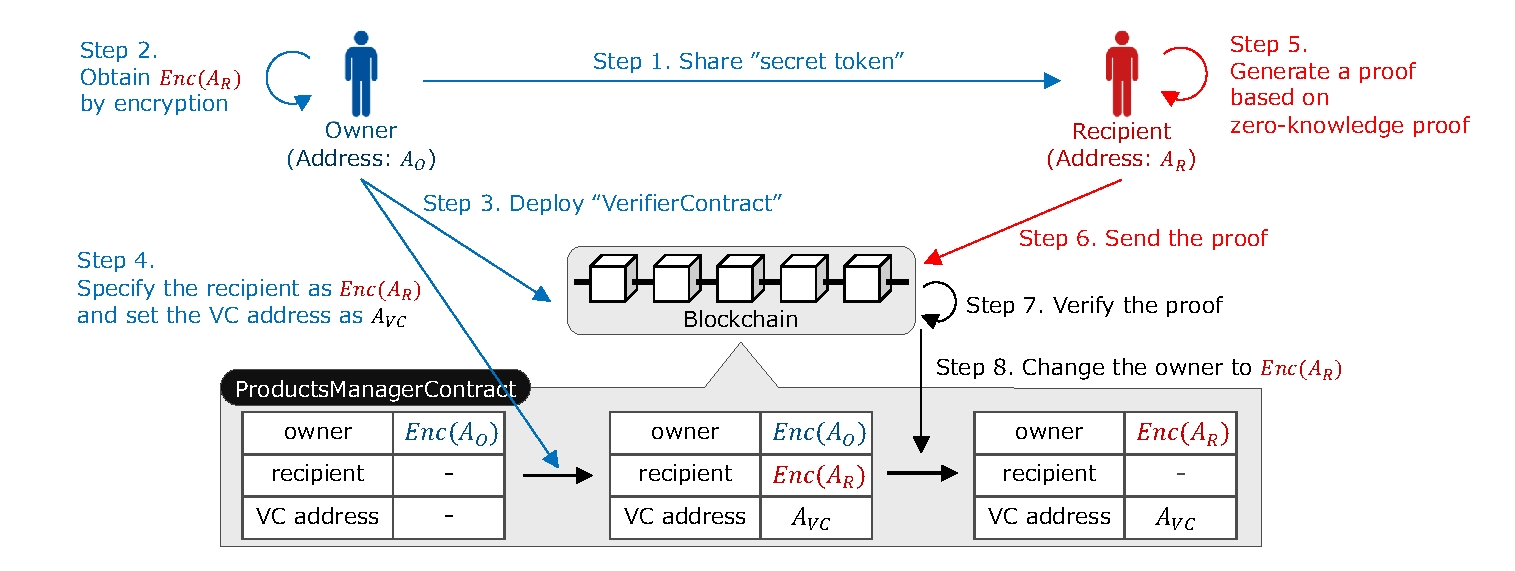
\includegraphics[width=0.8\textwidth]{flow.eps}
    \caption{Flow of distribution management in the proposed method.
    \label{fig:flow-ProposedMethod}}
\end{figure*}


\section{Verification}
\label{sec:verification}
% 攻撃者による不正行為を考慮し、提案手法の追跡性の担保とプライバシーの保護に関する検証を行なう。
We verify traceability and privacy of the proposed method by considering fraudulent activities by attackers.


\subsection{Traceability}
% 攻撃者が追跡性の担保を阻害する方法は、次の3つが考えられる。
There are three possible attack vectors for inhibiting traceability.
% 1つ目は、製造者以外の公開鍵を利用した暗号文をブロックチェーンに記録することで、製造者の秘密鍵による復号を妨げるものである。
% 提案手法では、Step7における検証の際、ブロックチェーンに記録されている製造者の公開鍵を直接参照して検証を実施する。
% そのため、製造者以外の公開鍵を利用した暗号文を記録すると、Step7の検証が常に失敗し、攻撃者による製品流通も失敗に終わる。
% よって、この攻撃は起こり得ない。
The first is to interfere with decryption of the owner's encrypted address using the manufacturer's private key.
This can be performed by the attacker recording an encrypted statement on the blockchain using a public key other than the manufacturer's.
However, the proof verification in Step~7 is performed by directly referring to the manufacturer's public key recorded in the blockchain.
% That is, recording a encrypted statement with a public key other than the manufacturer's will always fail to verify in Step 7, and product distribution by the attackers will also fail.
Therefore, the proof verification in Step~7 always fails if a statement encrypted with a public key other than the manufacturer's is recorded.
That is, distribution by an attacker also fails.
For this reason, it is impossible for this attack to succeed.

% 2つ目は、流通に関与しない第三者が、所有者もしくは受領者になりすますことで、不正な流通を行うというものである。
% これは、第三者が有効な証明を作成できてしまった場合に起こり得る。
% しかし、ゼロ知識証明の健全性から、証明に必要な情報を知らない者は有効な証明を作成することができない。そのため、なりすましは起こりえない。
The second attack vector is for a third party not involved in distribution to carry out %unauthorized distribution.
distribution by impersonating the owner or recipient.
This could happen if the third party is able to generate a valid proof.
However, those who do not know the information required for the proof cannot generate a valid proof because of the soundness of zero-knowledge proof.
Therefore, it is impossible for this attack to succeed.

% 3つ目は、所有者と受領者が結託し、無作為あるいは別の事業者のアドレスを暗号化したものをブロックチェーンに記録することで、所有者の特定を困難にするものである。
% 所有者と受領者が、Secret Tokenに加えて恣意的なアドレスを事前に共有し、それらを利用したゼロ知識証明を生成することで、PMCの所有者情報は正しく更新されてしまう。
% よって、攻撃は成功する。
% この攻撃への対応は今後の課題である。
The third attack vector is collusion between the owner and the recipient that makes it difficult to identify the owner.
This can be performed by the attacker using a random or real address other than his/her own.
The owner and recipient share an arbitrary address in addition to a secret token.
By using them to generate a proof, the owner information of \textit{PMC} is updated correctly. 
Therefore, it is possible for this attack to succeed.
We intend to deal with this attack in future work.
% Responding to this attack is a future work.

\subsection{Privacy}
% 攻撃者がプライバシーを侵害する方法は、ブロックチェーンに記録されている暗号文および証明情報から、流通に関与した者のアドレスを取得することである。
% まず暗号文について考察する。
% 暗号文の安全性は、使用する暗号鍵のビット長と計算方式に依存する。
% 例えば文献~\cite{bjj}の254ビットの楕円曲線暗号を利用する場合、秘密鍵を知らない者が、現実的な時間で暗号文を復号することは極めて困難である。
% そこで提案手法においても、文献~\cite{bjj}の暗号方式を利用することで、暗号文の安全性を担保できる。
% 次に、証明情報について考察する。
% 提案手法で使用するゼロ知識証明は、ゼロ知識性が保証されている。
% つまり、証明情報から、その証明の生成に利用したアドレスやSecret Tokenといった情報を復元することはできない。
% 以上の考察から、提案手法において、攻撃者がプライバシーを侵害することはできない。
An attacker can compromise privacy by retrieving the address from the owner's encrypted address or the proof recorded in \textit{PMC}.
First, we consider the encrypted address.
Cryptographic security depends on the key length and the cryptographic algorithm.
For example, when using 254-bit elliptic curve cryptography,  %\comu{proposed in}~\cite{bjj},
it is extremely difficult for a party who does not know the private key to decrypt the encrypted address in practical time.
Thus, we can ensure the security of the encrypted address in the proposed method by using the 254-bit elliptic curve proposed in~\cite{bjj}.
Second, we consider the proof used in the proposed method.
We use a zero-knowledge proof in the proposed method that is known to satisfy zero-knowledge-ness.
In other words, it is not possible to recover information such as the address and the secret token from the proof.
As a result, the attacker cannot compromise privacy.
That is, the attacker cannot retrieve the owner's blockchain address.


\section{Evaluation}
\label{sec:evaluation}
% 提案手法を Ethereum を用いて実装し、動作の検証を行う。
% また、その際のトランザクション手数料を算出し、結果に基づいたユースケースに関するディスカッションを行う。(discuss use cases based on evaluation results.)
To evaluate the proposed method, we implement it on the Ethereum platform. %the results of 
% its operation.
We also measure the transaction fees and discuss use cases based on the evaluation results.

\subsection{Environment setup}
% 評価では、ある1つの製品(a certain product)を、製造者を起点とし、6回流通させる。
% 製造者は製品の登録処理、発送処理を実行する。
% 製造者以外の流通者は、発送処理、受領処理を実行する。
We assume %that a given product is distributed six times, 
distributions of a %given 
product %,} 
starting with the manufacturer.
The manufacturer executes product registration and shipping operations.
The other %distributors
parties execute shipping and receiving operations.

% スマートコントラクトの記述には Solidity~\cite{Solidity} のバージョン 0.5.11 を使用する。
% 動作検証は、Remix~\cite{Remix}が提供するJavascriptVM環境を利用する。
% ゼロ知識証明に関連する実装には、zk-SNARKのツールボックスであるZoKrates~\cite{ZoKrates}を利用する。
We use Solidity version 0.5.11~\cite{Solidity} to write the smart contracts and the JavaScript Virtual Machine environment provided by Remix~\cite{Remix} to evaluate the %operational results of the proposed method.
proposed method.
% verify the operations.
We use ZoKrates~\cite{ZoKrates}, a toolbox of zk-SNARKs, for implementation of the zero-knowledge proof.

\begin{figure}[t]
    \centering
    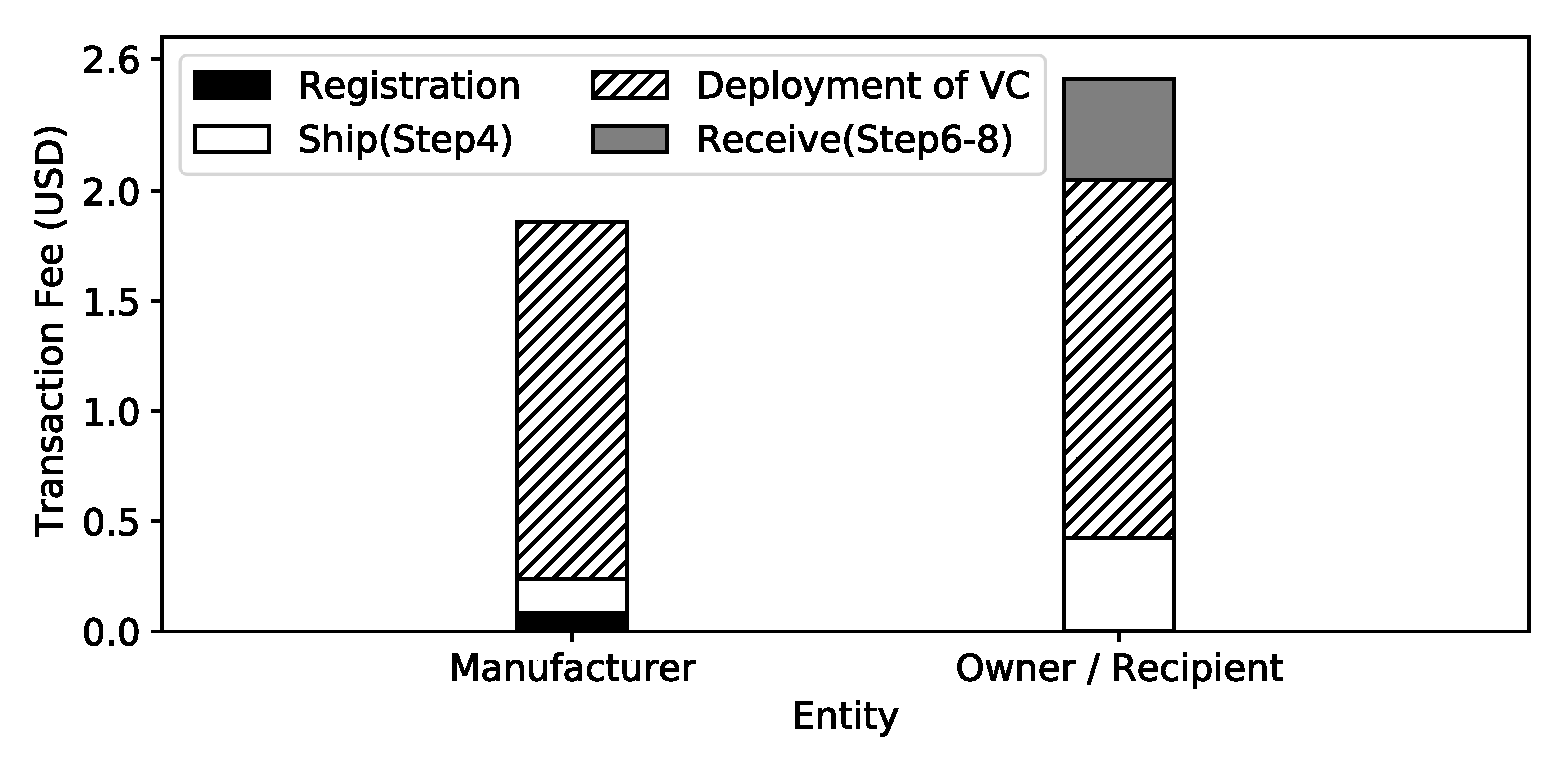
\includegraphics[width=0.43\textwidth]{graph.eps}
    \caption{Transaction fee per party for a certain product.\label{fig:evaluation}}
\end{figure}


\subsection{Result and Discussion}
% 6回の流通を終えた後に、MMC, PMC, VC に記録された情報から、アドレスが取得できないことを確認した。
% また、PMCに記録された所有者の暗号文を、製造者が自身の秘密鍵で復号することで、製品流通の所有者を特定することができることを確認した。
% ここから、提案手法では、プライバシーを担保しつつも製造者による追跡性を担保できることがわかった。
We found that the owner addresses could not be retrieved from the information recorded in %\textit{MMC}, 
\textit{PMC} and \textit{VC} after %six distributions.
distributions of a %given 
product.
We also confirmed that the manufacturer could identify the product owner by decrypting the owner's encrypted addresses recorded in \textit{PMC} using its own private key.
The proposed method can preserve privacy while 
securing traceability by the manufacturer.

% また、この流通に要したトランザクション手数料を算出した。
% なお、Remixが出力したgas値にgas priceを乗じることで、手数料ををUSDに換算する。
% 本評価を実施した2020年3月17日11時00分 (JST) 時点におけるgas priceは、1 gas = $1.1622 \times 10^{-6}$ USD であった。
% 製品流通における1人あたりに必要となるブロックチェーンのトランザクション手数料を、図~\ref{fig:evaluation}に示す。
% 製造者とそれ以外の流通者は、実行する処理が異なるため、必要なトランザクション手数料が異なる。
% 発送処理については、証明の検証作業の有無から、製造者と製造者以外の流通者が実行する関数の実装が異なる。そのため、同じ発送処理でもトランザクション手数料が異なる。
We measured the transaction fees for this distribution
and converted them into USD by multiplying the gas price by the gas value output by Remix.
At time of evaluation on March 17, 2020 at 11:00 a.m. (JST), the gas price was $1.1622 \times 10^{-6}$ USD per gas.
The maximum value of the transaction fee per party in this distribution is shown in \figurename~\ref{fig:evaluation}.
The manufacturer and the other %distributors
parties have different %required 
transaction fees because they execute different processes.
In addition, the shipping process has different implementations of the functions executed by the manufacturer and the other %distributors
parties, depending on whether the verification step is performed using the zero-knowledge proof.
% Therefore, the transaction fees differ according to the shipping process.
Therefore, the transaction fees of the shipping process differ between the manufacturer and the other %distributors
parties.

% 提案手法において、サプライチェーン上の1事業者もしくは1消費者が負担するトランザクション手数料の合計は、高々 2.6 USD であった。
% 実装の最適化を行なうことで手数料を削減できる余地はあるものの、現段階においても、車や家電製品といった高単価製品へ適用するユースケースが考えられる。
% このような製品は、製品に問題・欠陥があった場合、リコールの対象となる。
% 消費者へのリコールの周知活動の効率化およびリコール対象製品の回収率の低さは課題である~\cite{OECD2018}。
% 提案手法による流通であれば、製造者のみが製品の所在を特定できる。
% そのため、リコール対象の製品の所在を特定し、即座に保有者に通知を行なうことを通じて製品を回収することで、この課題を解決できる。
% 製品保有者からすると、高々 2.6 USDを支払うことによって、迅速に、修理や代替品への交換といった処置を受けることができる。
% この場合、トランザクション手数料を、このような保証を受けるための料金とみなすことができる。
% 2.6 USDであれば、保証を受けるための料金として高くない金額である。  
We found that the total transaction fees required for one party is at most 2.6 USD. 
Although there is room to reduce the fees by optimizing the implementation, there are still use cases that can be applied to high-priced products such as cars and home appliances even in the current implementation.
Such products are subject to recall if the product has a problem or defect.
The challenges of recalls include increasing consumer awareness of recalls and increasing recall response rates~\cite{OECD2018}.
In the case of distribution by the proposed method, only the manufacturer can track the product.
Therefore, these issues can be solved by tracking the product that is subject to recall and recalling that product through immediate notification of the owner.
The owner pays at most 2.6 USD to be able to promptly implement measures such as repair or replacement of the product. In this case, the transaction fee may be regarded as the fee for getting this kind of warranty and we believe that 2.6 USD is not an expensive charge for a warranty.



\section{Conclusions and Future Work}
\label{sec:conclusions}
% 本研究では、パブリックブロックチェーンを利用したサプライチェーンシステムにおいて、製品製造者による追跡性を担保しつつも、プライバシーを保護可能な手法を提案した。
% この手法をEthereumのスマートコントラクトに実装し、流通者あたりの手数料は高々2.6USDであることがわかった。
In this paper, we proposed a method that can preserve privacy while securing traceability by the product manufacturer in a supply chain system using PBC.
We implemented the proposed method on the Ethereum platform and found the transaction fee per party to be at most 2.6 USD.

% 今後の課題として、次の2つが挙げられる。
% 1つ目としては、トランザクション手数料を削減する方法の検討である。
% 提案手法のトランザクション手数料の多くは VC の登録処理が占めている。そこで、VCを所有者が流通のたびに登録するのではなく、製造者が事前に登録しておく。この事前に登録されたものを利用するような方法にすれば、VCの登録に関する手数料が1回分のみとなるため、手数料を大幅に削減が見込める。
% トランザクション手数料を削減することができれば、より安価な製品にも適用が可能となり、応用の幅が広がる。
% 2つ目としては、製品の加工・分解にも適用できるように、手法を拡張することである。
% 提案した手法では、単一の製品が形を変えずに流通することのみ、つまり完成品の流通のみを想定している。
% そのため、製品の加工・分解にも適用可能となれば、完成品以外の製品流通にも応用が可能となる。
There are two issues that remain to be addressed in the future.
The first issue is consideration of ways to reduce the transaction fees.
% The deployment of VC accounts for most of the transaction fee of the proposed method.
Most of the transaction fees in the proposed method arise from the deployment process of \textit{VC}.
Instead of the owner deploying \textit{VC} for each distribution, the manufacturer could deploy it in advance.
If %distributors
supply chain parties use a pre-deployed \textit{VC}, we can expect a significant reduction in the fees because of having only a one-time \textit{VC} deployment fee.
If the transaction fees can be reduced, we can apply this system to cheaper products.
The second issue is to extend the method so that it can be applied to the assembly and disassembly of products.
The proposed method assumes only the distribution of a single product without modification, that is, distribution of a finished product.
Therefore, if it could be applied to the assembly and disassembly of products, it could be applied to the distribution of products other than finished products.


%% ----------------------

% use section* for acknowledgement
% \section*{Acknowledgment}
% The authors would like to thank...

% trigger a \newpage just before the given reference
% number - used to balance the columns on the last page
% adjust value as needed - may need to be readjusted if
% the document is modified later
%\IEEEtriggeratref{8}
% The "triggered" command can be changed if desired:
%\IEEEtriggercmd{\enlargethispage{-5in}}

% references section

% can use a bibliography generated by BibTeX as a .bbl file
% BibTeX documentation can be easily obtained at:
% http://www.ctan.org/tex-archive/biblio/bibtex/contrib/doc/
% The IEEEtran BibTeX style support page is at:
% http://www.michaelshell.org/tex/ieeetran/bibtex/
\bibliographystyle{IEEEtran}
% argument is your BibTeX string definitions and bibliography database(s)
\bibliography{IEEEabrv, main}

\clearpage

% \section{コメント}

% \begin{itemize}
%     \item githubでのソースコード公開どうするか?
% \end{itemize}



% \section{今後の研究計画}
% \begin{itemize}
%     \item Crypto Valley Conference に short paper を投稿 (期限: 4/2)
%     \begin{itemize}
%         \item (3/7) IEEEの論文誌LaTeXスタイルをコンパイルする準備をoverleafで整える
%         \item (3/7) 論文で使用する図を選ぶ
%         \item (3/9) アブストを書く(in English)
%         \item (3/9) タイトルを書く(in English)
%         \item (3/10) 章構成を考える
%         \item (3/14) 上杉が日本語版初稿を完成
%         \begin{itemize}
%             \item (3/12) イントロ、関連研究
%             \item (3/13) Proposed Method
%             \item (3/14) Verification, Cost Evaluation, Conclusion
%         \end{itemize}
%         \item (3/14 or 15) 日本語版の添削による往復開始
%         \item (3/18) 村田先生に日本語版を添削依頼
%         \item (3/19) 村田先生の添削完了
%         \item (3/22) 上杉が英語版初稿を完成
%         \item (3/22 or 23) 英語版の添削による往復開始
%         \item (3/25) 英語版添削終了(後は校正にかけるだけの状態)
%         \item 英文校正にかける
%         \begin{itemize}
%             \item 見積もり・依頼 (3/25)
%             \item 納品 (3/31)
%         \end{itemize}
%     \end{itemize}
% \end{itemize}

\end{document}



